\documentclass{ucph-handout}
%\usepackage[english]{babel}

\usepackage{wrapfig}
\newcounter{handout}
\newcommand{\Ark}{Worksheet \arabic{handout}: }
\renewcommand{\Title}{\Ark Kickstart}%
\renewcommand{\TimeAndLocation}{DIKU, 2022}%
\renewcommand{\Author}{Martin Dybdal \& modified by DS}
\renewcommand{\AuthorEmail}{ds@di.ku.dk}

\begin{document}
% \chapter{Velkommen på datalogi!}
% Velkommen på datalogi og til kickstart-kurset i programmering!
% Nedenstående øvelser får jer hurtigt i gang med at programmere
% Python. Vi har med vilje udeladt at forklare en del ting, da vi gerne
% vil have jer selv til at eksperimentere jer frem.

%%==WORKSHEET 0
%
%\begin{exercisebox}[adjusted title=Første Program]
%Tast følgende eksempel ind i Processing editoren og tryk på
%\includegraphics[height=4mm]{illustrationer/processing_play_button}-knappen:
%\begin{python}
%size(400, 400)
%
%# Træ
%rect(55, 50, 10, 20)
%ellipse(60, 35, 30, 40)
%\end{python}
%Tilføj derefter:
%\begin{python}
%# Kraftværk
%rect(120, 50, 60, 30)
%rect(160, 20, 10, 30)
%triangle(120, 50, 136, 40, 136, 50)
%triangle(136, 50, 152, 40, 152, 50)
%\end{python}
%Og:
%% \begin{python}
%% # Person
%% ellipse(270, 65, 8, 8)
%% line(270, 70, 270, 75)
%% line(270, 69, 277, 75)
%% line(270, 69, 263, 75)
%% line(270, 75, 275, 82)
%% line(270, 75, 265, 82)
%% \end{python}
%\begin{python}
%# Vindmølle
%line(300, 50, 320, 51)
%line(300, 50, 289, 67)
%line(300, 50, 291, 32)
%line(300, 50, 300, 90)
%\end{python}
%
%\tcbsubtitle{Prøv nu at tegne en bil og en sky:}
%\includegraphics[width=0.4\textwidth]{illustrationer/bil-streg.png}
%\includegraphics[width=0.3\textwidth]{illustrationer/sky.png}
%\end{exercisebox}
%
%\begin{exercisebox}[adjusted title=Farver]
%I skal nu farvelægge figurerne. Til det skal I bruge
%\ttpy{fill(r, g, b)}-funktionen, der vælger hvilken farve der skal
%bruges til udfyldning og tekstfarve. Det handler om at kalde
%\ttpy{fill} de rigtige steder! Som argumenter angiver man mængden
%af rød (0-255), blå (0-255) og grøn (0-255).
%
%~
%
%\noindent
%Her er nogle grundfarver:
%
%\begin{minipage}{0.45\linewidth}
%\begin{python}
%fill(255, 0, 0)  # rød
%fill(0, 255, 0)  # grøn
%fill(0, 0, 255)  # blå
%\end{python}
%\end{minipage}
%\begin{minipage}{0.45\linewidth}
%\begin{python}
%fill(0, 0, 0)       # sort
%fill(255, 255, 255) # hvid
%fill(255, 255, 0)   # gul
%\end{python}
%\end{minipage}
%
%\noindent
%Find eventuelt farver ved hjælp af en online farvevælger eller RGB
%farve tabel. Søg for eksempel efter ``rgb color picker''.
%\tcbsubtitle{Streger og omrids:}
%Til at angive farven på streger (fx \ttpy{line}) og omrids
%bruges \ttpy{stroke(r, g, b)}. Prøv også funktionen \ttpy{noStroke()},
%til at slå optegning af omrids fra.
%\end{exercisebox}
%
%\newpage
%\begin{exercisebox}[adjusted title=Eksempel]
%\noindent
%Her er et eksempel på hvordan det kan se ud efter farvelægning:
%\begin{center}
%\includegraphics[width=0.55\textwidth]{illustrationer/farvelagt.png}
%\end{center}
%\end{exercisebox}
%
%\begin{exercisebox}[adjusted title=Green City]
%%Gem projektet og giv det navnet ``Elbil''. Senere skal vi udbygge dettil en simulation hvor bilen skal lades med strøm fra enten vindmølleeller kraftværket, men hvor bilen helst skal lades op med grøn strøm fra vindmøllen.
%
%Brug det I har lært til at få det til at blive en lidt pænere scene, med baggrund, forgrund og de ekstra detaljer som I synes der skal være der. Jeg har fx tegnet en vej og flyttet lidt rundt på figurerne. 
%\\
%\\
%\textbf{Tip: }For at ændre baggrundsfarven fra grå  kan i bruge \ttpy{rect} som i
%allerede kender, men i kan også bruge kommandoen \ttpy{background(r, g, b)}.
%Den sletter alt og udfylder skærmen med den angivne farve.
%
%\begin{center}
%\includegraphics[width=0.55\textwidth]{illustrationer/elbil.png}
%\end{center}
%
%\noindent
%Husk at bruge kommentarer, så I nemt kan finde rundt i koden!
%\end{exercisebox}
%
%%==WORKSHEET 1
%
%\newpage
%\stepcounter{handout}
%\begin{exercisebox}[adjusted title=Variable]
%Opret et nyt projekt (``File'' -> ``New'') og gem med det samme
%projektet. Kald det ``Akvarie''.
%
%\noindent
%Skriv denne stump kode ind:
%\begin{python}
%size(400, 400)
%fishX = 150
%ellipse(fishX, 200, 120, 75)
%triangle(fishX - 60, 200, fishX - 90, 170, fishX - 90, 230)
%\end{python}
%Prøv at ændre 150 til et andet tal i angivelsen af \ttpy{fishX}.\\
%
%\noindent
%Tilføj nu følgende:
%\begin{python}
%eyeSize = 15
%ellipse(fishX + 30, 190, eyeSize, eyeSize)
%\end{python}
%Prøv at ændre på værdien af \ttpy{eyeSize}.
%
%\tcbsubtitle{Opgaver:}
%\noindent
%I har nu tilføjet en fisk der kan flyttes, bare ved at ændre én
%værdi.
%
%\begin{itemize}
%\item Farvelæg fisken
%\item Giv fisken en finne, som flytter med når I ændrer \ttpy{fishX}.
%\item Giv fisken en pupil, som flytter med når I ændrer \ttpy{fishX}.
%\item Lav en ny variabel, \ttpy{fishY}, der styrer fiskens y-position
%\end{itemize}
%\hspace{1cm}\includegraphics[width=0.4\textwidth]{illustrationer/fisk-fishY.png}
%
%\noindent
%Husk at gemme projektet. Vi skal arbejde videre med det senere.
%missing link
%\end{exercisebox}
%\newpage
%\begin{exercisebox}[adjusted title= Green City forstat]
%Skift over til elbil-projektet og indfør variable til angivelse af
%objekternes placering, så vi senere kan animere objekterne.
%
%\begin{itemize}
%\item Lav en variabel \ttpy{carX} så bilen kan bevæge sig frem
%  og tilbage
%\item Lav en variabel \ttpy{cloudX} så skyen kan bevæge sig frem og tilbage
%\item Lav en variabel \ttpy{treeX} så træet kan flyttes horizontalt
%\item Lav en variabel \ttpy{treeY} så træet kan flyttes vertikalt
%\end{itemize}
%\begin{center}
%\includegraphics[width=0.5\textwidth]{illustrationer/carX-cloudX-treeXY.png}
%\end{center}
%\end{exercisebox}
%
%\begin{exercisebox}[adjusted title=Akvarie fortsat]
%Brug nu det I har lært til at udvide akvarie projektet, her er et
%eksempel, men brug gerne jeres fantasi! Der er fx brugt en variabel
%til x-koordinat af tangplanten, og en anden variabel til x-koordinat
%af hele gruppen af sten (som en enhed). Der er oprettet et ekstra sæt
%variable \ttpy{fish2X}/\ttpy{fish2Y} til at styre placeringen af den
%ekstra fisk.%  Man kunne også forestille sig bobler, et mini sandslot,
%% andre tangplanter, muslingeskaler eller andre dyr.
%
%\begin{center}
%\includegraphics[width=0.4\textwidth]{illustrationer/akvarie.png}
%\end{center}
%
%\end{exercisebox}

%==WORKSHEET 2 
\newpage
\stepcounter{handout}

\begin{exercisebox}[adjusted title = Funktioner]
Funktioner giver mulighed for at genbruge den samme kode flere steder,
navngive hele blokke af kode og sætte struktur på kode.\\

\noindent
Åbn akvarie-projektet. Tilføj følgende ``fiske-tegne-funktion''
nederst i projektet. BEMÆRK! Linjeindrykning med 4 mellemrum er vigtig!

\begin{python}
def drawSimpleFish(x, y):
    ellipse(x, y, 120, 75)
    triangle(x - 60, y, x - 90, y - 30, x - 90, y + 30)

drawSimpleFish(100,  50)
drawSimpleFish(300, 200)
drawSimpleFish(20, 20)
drawSimpleFish(80, 80)
\end{python}
Nu går det meget hurtigere med at få fyldt akvariet med fisk, og vi
undgår at kopiere kode.

\tcbsubtitle{Opgaver:} Opret jeres egen \ttpy{drawFish(x, y)} funktion, der tegner hele jeres
fisk med farve, finner og øjne.

begin{exercisebox}[adjusted title= Green City forstat ]
Ovre i elbil-projektet kan I også prøve at skrive en funktion
til at tegne træer:
\begin{python}
def drawTree(treeX):
    fill(100, 100, 0)
    rect(treeX - 5, 350, 10, 20)
    fill(0, 200, 0)
    ellipse(treeX, 335, 40, 50)

drawTree(160)
drawTree(300)
\end{python}

\noindent
Få sat struktur på koden til elbil-projektet ved hjælp af funktioner:
\begin{itemize}
\item Skriv en \ttpy{drawCloud(x)}-funktion der tegner en sky
\item Udvid \ttpy{drawTree(x)}-funktionen til at også tage imod et y-koordinat
\item Skriv en \ttpy{drawCar(x)}-funktion der tegner en bil
\item Skriv en \ttpy{drawPowerplant()}-funktion og en
  \ttpy{drawWindmill()}-funktion, der tegner hhv. kraftværket og
  vindmøllen. Vi får ikke behov for at flytte på dem, så de behøver
  ikke tage koordinater som argument.
\end{itemize}

\noindent
Kald alle funktionerne nederst i dit program. For eksempel:

\begin{python}
drawTree(150, 235)
drawTree(240, 335)
drawPowerplant()
drawWindmill()
drawCar(50)
drawCloud(280)
\end{python}
\end{exercisebox}

% == Worksheet 3
%\newpage
%~
\newpage
\stepcounter{handout}
\begin{exercisebox}[adjusted title= Animation og funktionerne]% \ttpy{setup}/\ttpy{draw}]

Opret et nyt midlertidigt projekt (I behøver ikke gemme det). Tast
denne stump kode ind:
\begin{python}
x = 50
  
def setup():
    size(400, 400)

def draw():
    global x
    background(255, 255, 255)
    fill(255, 0, 0)
    ellipse(x, 100, 30, 30)
    x = x + 1
\end{python}

\noindent
Funktionen \ttpy{draw} kaldes automatisk 60 gange i sekundet!

\tcbsubtitle{Opgaver:}
\begin{itemize}
\item Prøv at ændre $50$ til et andet tal 
\item Prøv at ændre linjen \ttpy{x = x + 1} til \ttpy{x = x - 1} eller til \ttpy{x = x + 5}
\item Forsøg at flytte kaldet til \ttpy{background} fra \ttpy{draw}
  til \ttpy{setup} - hvad sker der?
\end{itemize}


\tcbsubtitle{BEMÆRK!!:} 
Når man bruger
\ttpy{setup}/\ttpy{draw}~ er det ikke tilladt at kalde
tegne-funktioner udenfor \ttpy{setup} og
\ttpy{draw}, alt skal flyttes ind i de to funktioner.

\end{exercisebox}

\begin{exercisebox}[adjusted title= Akvarie fortsat]
\begin{itemize}
\item \emph{Omskrivning af akvarieprojektet til brug af \ttpy{setup}/\ttpy{draw}:}
  \begin{itemize}
   \item Tilføj tomme \ttpy{setup} og \ttpy{draw}-funktioner nederst i programmet
    \item Kald \ttpy{size(400, 400)} i \ttpy{setup}
     \item Kald alle tegnefunktionerne i \ttpy{draw}, inkl. tegning af baggrunden
  \end{itemize}
  
\item \emph{Få fiskene til at svømme:}
  \begin{itemize}
  \item Opret to globale variabler \ttpy{fish1X} og
  \ttpy{fish2X} (før \ttpy{setup}/\ttpy{draw})
  \item Brug de nye variable som x-argument når I kalder \ttpy{drawFish()}
  \item \emph{HUSK} linjerne: ~\ttpy{global fish1X}~ og ~\ttpy{global fish2X}~
  \item Opdater variablerne med $+1$/$-1$ inde i \ttpy{draw}-funktionen
  \end{itemize}
\end{itemize}
\end{exercisebox}

\begin{exercisebox}[adjusted title= Green City forstat]
\begin{itemize}
\item Opret to globale variabler \ttpy{carX} og \ttpy{cloudX}
\item Få bilen til at køre mod højre
\item Få skyen til at starte uden for billedet i højre side og bevæge sig mod venstre
\end{itemize}
\end{exercisebox}


%%\emph{TODO: illustrationer}
\begin{exercisebox}[adjusted title= Tilfældighed]
Opret et helt nyt projekt, gem det som ``random\_circles''. Tilføj følgende kode:
\begin{minipage}{0.60\linewidth}
\begin{python}
def setup():
    size(400, 400)

def draw():
    x = random(0, width)
    y = random(0, height)
    ellipse(x, y, 30, 30)
\end{python}
\end{minipage}

\begin{minipage}{0.40\linewidth}
\includegraphics[width=0.70\textwidth]{illustrationer/randomcircles.png}
\end{minipage}
~
\end{exercisebox}

%\begin{minipage}{0.45\textwidth}
%\begin{Right}

%\end{Right} \end{minipage}

\begin{exercisebox}[adjusted title=Opgaver: ]


\begin{itemize}
\item Få cirklerne til at ændre størrelse tilfældigt
\item Få cirklerne til at blive tegnet i tilfældige
  farver. Eksperimenter jer frem til en farveskala I synes er pæn.
\end{itemize}

\end{exercisebox}

\begin{exercisebox}[adjusted title=Input fra musen]
Placeringen af musen kan aflæses med variablerne \ttpy{mouseX}
og \ttpy{mouseY}. En slags tegneprogram kan skrives således:
\begin{python}
def setup():
    size(800, 800)
    background(255, 255, 255)

def draw():
    fill(0, 0, 0)
    ellipse(mouseX, mouseY, 5, 5)
\end{python}
\end{exercisebox}

\begin{exercisebox}[adjusted title=Tastatur input]
%\chapter{Tastatur input}
Åbn tegneprograms-projektet og prøv at tilføje følgende nye funktion:
\begin{python}
def keyPressed():
    background(255, 255, 255)
\end{python}
Start programmet og tryk på en vilkårlig tast på tastaturet. For at
tjekke efter en specifik tast kan variablen ``\ttpy{key}'' aflæses.
\begin{python}
def keyPressed():
    if key == 'c':
        background(255, 255, 255)
\end{python}
%NEED FOOTNOTE
\end{exercisebox}

\begin{exercisebox}[adjusted title=Nyt projekt: Kreativt tegneprogram ]
Opgaven er nu at lave et tegneprogram der er mere kunstfærdigt. Tegn
linjer fra alle hjørner og midtpunkter på siderne. Brug
variablerne \ttpy{width} og \ttpy{height}.
\begin{center}
  \includegraphics[width=0.40\textwidth]{illustrationer/kryds.png}
  \quad
  \includegraphics[width=0.40\textwidth]{illustrationer/kryds-tegning.png}
\end{center}
Husk at gemme projektet!
\end{exercisebox}

%%==WORKSHEET #4
%\newpage
%\stepcounter{handout}
%\begin{exercisebox}[adjusted title= Betingelser]
%Med betingelser kan vi få ting til at ske når specielle kriterier er
%opfyldt. Åbn akvarie-projektet og prøv at indsætte følgende i
%\ttpy{draw}-funktionen:
%\begin{python}
%if fish1X > 500:
%    fish1X = -40
%        
%if fish1X < -50:
%    fish1X = 450
%\end{python}
%\noindent
%Hvad sker der?
%\end{exercisebox}
%
%\begin{exercisebox}[adjusted title= Skifte retning]
%Ved at lave en variabel der indeholder retningen som fisken svømmer,
%kan vi få den til at ændre retning når den når siderne.
%
%\begin{itemize}
%\item Definer en global variabel \ttpy{fish1XVelocity} og sæt den til $1$
%\item Ændr \ttpy{fish1X = fish1X + 1} til \ttpy{fish1X = fish1X + fish1XVelocity}
%\item Fjern den tidligere \ttpy{fish1X}-betingelse
%\item Tilføj disse betingelser:
%\begin{python}
%if fish1X > 400:
%    fish1XVelocity = -1
%if fish1X < 0:
%    fish1XVelocity = 1
%\end{python}
%\end{itemize}
%\end{exercisebox}
%
%\begin{exercisebox}[adjusted title=Ændre udseende ]
%%\chapter{Ændre udseende}
%Prøv at ændre \ttpy{drawFish}-funktionen, så den tager retningen af
%fisken med som argument, og brug en betingelse til at tegne finner og
%øjne forskelligt alt efter hvilken retning fisken svømmer.
%
%\begin{minipage}{0.60\linewidth}
%\begin{python}
%def drawFish(x, y, eyeSize, velocity):
%    ... tegn kroppen ...
%
%    # Svømmer mod højre
%    if velocity >= 0:
%        ... tegn finner og øjne ...
%
%    # Svømmer mod venstre
%    if velocity < 0:
%        ... tegn finner og øjne ...
%\end{python}
%\end{minipage}
%\begin{minipage}{0.40\linewidth}
%\includegraphics[width=0.70\textwidth]{illustrationer/fisk-begge-retninger.png}
%\end{minipage}
%~
%\end{exercisebox}
%\begin{exercisebox}[adjusted title=Gør akvarieprojektet færdigt ]
%Nu er vi sådan set færdig med akvarie-projektet. Tilføj eventuelt
%flere elementer. F.eks. bobler der dukker op fra bunden og svømmer mod
%overfladen.
%\end{exercisebox}
%
%%\newpage
%%
%\begin{exercisebox}[adjusted title=Flere opgaver om betingelser]
%Åbn Green City projekt og gør følgende:
%\begin{itemize}
%\item Få skyen til at flytte tilbage til start og komme forbi igen og
%  igen, hver gang den rammer kanten
%\item Få bilen til at vende om i begge ender.
%\end{itemize}
%\tcbsubtitle{Opgaver:}
%Bilen skal stoppe når batteriet er tomt
%  \begin{itemize}
%  \item Definer en global variabel \ttpy{carBattery} og sæt den til 100
%  \item Reducer den med 0.1 hver gang \ttpy{draw} kaldes
%  \item Vis batteriets status vha. \ttpy{text(string, x, y)}-funktionen.
%    Husk at konvertere tallet til en string vha. \ttpy{str()}.
%  \item Hvis batteriet er tomt (\ttpy{<= 0}) skal bilen stoppe (sæt velocity til 0)
%  \end{itemize}
%Tilføj en  \ttpy{keyPressed()} -funktion og gør så man kan oplade elbilen, når man trykker 'C':
%  \begin{itemize}
%  \item Læg \ttpy{0.3} til \ttpy{carBattery}, hver gang der tykkes 'C' på tasturet
%  \item Hvis \ttpy{carBattery} overstiger 100, så sæt den til 100, så man kan ikke lade til mere end 100\%
% \end{itemize}
%\end{exercisebox}
%
%
%%\chapter{Tastatur input}
%%Åbn tegneprograms-projektet og prøv at tilføje følgende nye funktion:
%%\begin{python}
%%def keyPressed():
%%    background(255, 255, 255)
%%\end{python}
%%Start programmet og tryk på en vilkårlig tast på tastaturet. For at
%%tjekke efter en specifik tast kan variablen ``\ttpy{key}'' aflæses.
%%\begin{python}
%%def keyPressed():
%%    if key == 'c':
%%        background(255, 255, 255)
%%\end{python}
%%Skift nu over til elbilsprojektet og brug det du lige har lært, så man
%%kan oplade bilen når man trykker 'C':
%%\begin{itemize}
%%  \item Læg \ttpy{0.3} til \ttpy{carBattery} hver gang der
%%    trykkes C
%%  \item Hvis \ttpy{carBattery} overstiger 100, så sæt den til
%%    100, så man ikke kan lade til mere end 100\%
%%\end{itemize}
%
%\begin{exercisebox}[adjusted title= Skftiende vindhastighed]
%Variablen \ttpy{frameCount} tæller hvor mange gange \ttpy{draw} er
%kørt siden programmet startede. Indtast dette i draw-funktionen i
%elbil-projektet:
%\begin{python}
%fill(0, 0, 0)
%text(frameCount, 350, 20)
%if frameCount % 60 == 0:
%    print(frameCount)
%\end{python}
%
%%new stuff
%
%
%\noindent
%Eftersom \ttpy{draw} udføres med \textit{60 frames per second}, vil
%\ttpy{print}-funktionen blive udført hvert sekund.
%
%\vspace{2mm}
%\noindent
%Det kan vi også bruge i elbilsprojektet, til at opdatere
%vindhastigheden hvert sekund.
%  \begin{itemize}
%  \item Opret en global windSpeed variabel
%  \item Opdater windSpeed med en ny tilfældig værdi hvert sekund
%  \item Vis vindhastigheden vha. \ttpy{text()}
%  \end{itemize}
%% \item Tænd og sluk for kraftværket
%   \begin{itemize}
%   \item Opret en global variabel \ttpy{powerplantOn}
%   \item Gør så man kan tænde og slukke kraftværket med en tryk på 'p'
%   \item Tegn røgskyer over kraftværket når det er tændt
%   \item Opret en variabel \ttpy{co2emission} og læg lidt til så længe
%     kraftværket er tændt. Vis værdien med \ttpy{text()}
%   \end{itemize}
%\end{exercisebox}

%\newpage
%\stepcounter{handout}
%\chapter{Tilstandsmaskiner (Finite state machines)}
%\begin{minipage}{1.0\linewidth}
%\begin{wrapfigure}[9]{r}{0.15\textwidth}
%    \vspace{-1em}
%    \includegraphics[width=0.15\textwidth]{illustrationer/unitek_kombinationslaas.jpg}
%\end{wrapfigure}
%  
%Som det første eksempel på en tilstandsmaskine skal vi lave en
%elektronisk kombinationslås, som dem der bruges til adgangskontrol på
%døre.
%
%\noindent
%Tilstandsdiagram:
%
%\noindent
%\includegraphics[width=0.85\textwidth]{graphviz/combinationLock_dumb}
%
%Hent Processing.py koden til kombinationslåsen her:
%\mbox{\url{http://kortlink.dk/ufdh}} og kopier den ind i et nyt Processing-projekt.
%
%% Indtast følgende kode:
%% \begin{python}
%% lockState = "LOCKED"
%
%% def setup():
%%     size(400, 400)
%
%% def draw():
%%     background(255, 255, 255)
%%     fill(0)
%%     text(lockState, 20, 20)
%
%% def keyPressed():
%%     global lockState
%%     if lockState == "LOCKED":
%%         if key == '3':
%%             lockState = "FIRST_CORRECT"
%%         else:
%%             lockState = "LOCKED"
%%     elif lockState == "FIRST_CORRECT":
%%         if key == '2':
%%             lockState = "SECOND_CORRECT"
%%         else:
%%             lockState = "FIRST_CORRECT"
%%     elif lockState == "SECOND_CORRECT":
%%         if key == '6':
%%             lockState = "UNLOCKED"
%%         else:
%%             lockState = "SECOND_CORRECT"
%% \end{python}
%\end{minipage}
%
%\begin{itemize}
%\item  Afprøv kombinationslåsen og følg med som tilstanden skifter. Hvis man
%ikke kendte løsenet (passwordet), hvor mange forsøg kræver det så
%at gætte sig frem?
%
%\item Ændr koden, så løsenet i stedet er 524
%\item Prøv at ændre koden til at følge dette diagram i stedet, hvor
%  forkerte tryk sætter tilstanden tilbage til start:
%  
%\includegraphics[width=0.85\textwidth]{graphviz/combinationLock_resetting}
%
%\item Tegn et udvidet tilstandsdiagram over kombinationslåsen, med en ekstra
%  tilstand, så der kræves 4 cifre. Tilføj dernæst den ekstra tilstand i koden.
%\end{itemize}
%
%\chapter{Automatisk genlås efter 2 sekunder}
%Lad os udvide låsen, så døren automatisk låser igen efter 2 sekunder,
%hvilket svarer til 120 frames:
%
%\noindent
%\begin{center}
%\includegraphics[width=1.0\textwidth]{graphviz/combinationLock_timeout}
%\end{center}
%
%\begin{itemize}
%\item Opret en global variabel ``\ttpy{timer}'' og sæt den til 0
%\item Sæt \ttpy{timer}-variablen til 120 så snart låsen bliver låst op, det vil
%  sige når den skifter \ttpy{lockState} til \ttpy{"UNLOCKED"}.
%\item Tæl ned med timeren i hver frame (tilføj følgende til \ttpy{draw}-funktionen):
%\begin{python}
%global timer
%if timer > 0:
%    timer = timer - 1
%\end{python}
%\item Når timeren er talt helt ned, skal låsen åbnes. I
%  \ttpy{draw}-funktionen skal I nu tjekke om vi er i tilstanden
%  \ttpy{"UNLOCKED"} og timeren samtidig er talt ned til 0. Indsæt
%  følgende i \ttpy{draw}:
%\begin{python}
%if lockState == "UNLOCKED":
%    if timer == 0:
%        lockState = "LOCKED"
%\end{python}
%\end{itemize}
%
%\chapter{Alarm}
%Et andet eksempel på en tilstandsmaskine er en tyverialarm. Den har
%tre tilstande ``DEAKTIVERET'', ``AKTIV'' og ``ALARM''. Her er
%tilstandsdiagrammet:
%
%\noindent
%\includegraphics[width=1.0\textwidth]{graphviz/alarm}
%
%\noindent
%Opret et nyt projekt og indtast koden herunder. Den indeholder
%funktionalitet til at opdage et indbrud, ``bevægelse registreret'' i
%figuren ovenfor. Det sker når man bevæger musen ind i cirklen i
%midten.
%\begin{python}
%alarmState = "DEAKTIVERET"
%
%def setup():
%    size(400, 400)
%
%def draw():
%    global alarmState
%    background(255, 255, 255)
%    fill(0)
%    text(alarmState, 20, 20)
%    text("Slaa alarmen til/fra ved at trykke 's'", 20, 40)
%
%    noFill()
%    ellipse(200, 200, 100, 100)
%
%    if alarmState == "AKTIV":
%        # Tjek om musens cursor er inde i cirklen
%        if dist(mouseX, mouseY, 200, 200) < 50:
%            alarmState = "ALARM"
%    elif alarmState == "ALARM":
%        text("Indbrud", 20, 60)
%
%def keyPressed():
%    # indtast kode til at slå alarmen til/fra her
%\end{python}
%
%\noindent
%Det er nu din opgave at tilføje de sidste dele der gør det muligt at
%slå alarm til/fra og at alarmen stopper automatisk efter en timeout.
%\begin{itemize}
%\item \emph{Slå til/fra:} Tilføj en \ttpy{keyPressed} funktion der tillader at slå alarmen
%  til og fra når der trykkes 's'
%% \item Ændr koden i \ttpy{draw()} så alarmens tilstand sættes til ALARM, når musen er
%%   inde i cirklen OG tilstanden er AKTIV, i stedet for at der bare
%%   skrives ``Indbrud'' på skærmen.
%\item \emph{Time out:} Tilføj en timer, der sættes til 180 (3
%  sekunder) når alarmen går i gang, og som slår alarmen fra igen når
%  den er nede på 0 (dvs. sætter alarmState til \ttpy{"AKTIV"}).
%\end{itemize}
%
%
%\newpage
%\stepcounter{handout}
%\chapter{Elbil-projektet - de sidste dele}
%Vi skal nu bruge en tilstandsmaskine til at få afsluttet
%elbilprojektet, men det kommer til at tage nogle skridt. Først skal vi
%have omskrevet logikken i bilen til at bruge en tilstandsmaskine i
%stedet for ``carXVelocity''. Vi har lige nu 3 tilstande:
%\begin{itemize}
%\item \ttpy{"FORWARD"} - bilen kører mod højre
%\item \ttpy{"BACKWARD"} - bilen kører mod venstre
%\item \ttpy{"OUT_OF_FUEL"} - bilen er løbet tør for strøm og spillet er slut
%\end{itemize}
%\begin{center}
%\includegraphics[width=1.2\textwidth]{graphviz/carStateMachine_simple}
%\end{center}
%
%\begin{itemize}
%\item Når vi er i FORWARD tilstanden, flyttes bilen fremad, batteriet
%  mister strøm
%\item Når vi er i BACKWARD tilstanden flyttes bilen bagud, batteriet mister strøm
%\item Når vi er i OUT\_OF\_FUEL tilstanden skal der ikke ske noget. Spillet er slut.
%\end{itemize}
%
%\noindent
%Koden skal have følgende struktur. Din opgave er at udfylde ``...''
%med koden der flytter bilen, skifter tilstand og bruger strøm fra
%batteriet.
%\begin{python}
%    if carState == "FORWARD":
%        ...
%        if carX > 400:
%            ...
%        if carBattery <= 0:
%            ...
%    elif carState == "BACKWARD":
%        ...
%        if carX < 0:
%            ...
%        if carBattery <= 0:
%            ...
%    elif carState == "OUT_OF_FUEL":
%        pass # pass means "do nothing"
%\end{python}
%
%\newpage
%\chapter{Udvidet tilstandsmaskine}
%Vi skal nu have gjort så bilen parkerer hver gang den når venstre side
%af skærmen. Derfor udvider vi vores tilstandsmaskine med en
%parkeringstilstand:
%\begin{center}
%\includegraphics[width=1.2\textwidth]{graphviz/carStateMachine_parking}
%\end{center}
%
%\noindent
%Samtidig skal der ske noget når vi skifter tilstand:
%\begin{itemize}
%\item Når vi skifter tilstand fra BACKWARD til PARKING, skal vi sætte
%  en timer. Det gør vi ved at sætte en global variabel carParkingTimer
%  til 600 (10 sekunder).
%\item Når vi er i PARKING tilstanden trækker vi en fra carParkingTimer
%  i hver iteration af draw.
%\end{itemize}
%
%\chapter{Kun opladning når der er parkeret}
%Den sidste udvidelse af tilstandsmaskinen gør at vi kun kan oplade
%bilen imens vi er parkeret.
%
%\hspace{-3cm}
%\includegraphics[width=1.5\textwidth]{graphviz/carStateMachine_charging}
%
%\noindent
%Der tilføjes tre skift mellem tilstande:
%\begin{itemize}
%\item Tilstanden skifter frem og tilbage mellem PARKING og CHARGING
%  når der trykkes på tasten 'c'
%\item Når man er i CHARGING tilstanden, skal bilen også begynde at
%  køre igen når \ttpy{carParkingTimer} er 0.
%\end{itemize}
%
%\noindent
%Samtidig skal der tilføjes kode så bilen lader automatisk så længe
%\ttpy{carState == CHARGING}.
%
%\chapter{CO2 udledning}
%Den sidste del af projektet er at få CO2-udledningen til at afhænge af
%vindhastigheden. Vi opretter en global variabel \ttpy{totalEmission}
%og sætter den til:
%\begin{python}
%if carState == "CHARGING":
%    totalEmission = totalEmission + 4 - windSpeed
%\end{python}
%
%\noindent
%Når windSpeed er 4 m/s vil der derfor ikke forurenes, når windSpeed er
%3 vil derforurenes en lille smule og så videre.
%
%
%% \newpage
%% \stepcounter{handout}
%% \chapter{Objekter}
%% Med objekter kan vi gruppere mange værdier sammen. Vi skal nu lave
%% fiske-objekt der gemmer alle værdierne om en fisk (x, y, hastighed,
%% øjenstørrelse).
%
%% \begin{python}
%% def makeFish(x, y, velocity, eyeSize):
%%     return { "x" : x,
%%              "y" : y,
%%              "velocity" : velocity,
%%              "eyeSize" : eyeSize }
%
%% fish1 = makeFish(200, 50, 1, 15)
%% print(fish1)
%% print(fish1["x"])
%% print(fish1["y"])
%% print(fish1["velocity"])
%% print(fish1["eyeSize"])
%% \end{python}
%
%% \begin{python}
%% def drawFish(fish):
%%     x = fish["x"]
%%     y = fish["y"]
%%     velocity = fish["velocity"]
%%     eyeSize = fish["eyeSize"]
%%     ... tegne kommandoer som tidligere ...
%
%% def moveFish(fish):
%%     fish["x"] = fish["x"] + 1
%% \end{python}
%
%
%
%% \newpage
%% \stepcounter{handout}
%% \chapter{Rotation i Processing.py}
%% Hvis vi gerne vil rotere en tegning i Processing, så gøres det via et
%% par kommandoer til at ændre hele koordinatsystemet.
%
%% \chapter{Flyt origo, (0,0)}
%% Med kommandoen \ttpy{translate(x,y)}, kan vi ændre hele
%% koordinatsystemet, så vi kan tegne med origo et andet sted end øverst
%% til venstre (med andre ord: flytte hvor vi har koordinat $(0,0)$).
%% \begin{python}
%% translate(150, 100)
%% ellipse(0, 0, 120, 75)
%% triangle(-60, 0, -90, -30, -90, 30)
%% \end{python}
%
%% \chapter{Roter koordinatsystemet}
%% Rotation af koordinatsystemet gøres med kommandoen \ttpy{rotate(rad)} og
%% det påvirker så alt der tegnes efterfølgende. Rotationen foregår rundt
%% om origo, og derfor vil man oftest først bruge translate til at flytte
%% hen til det punkt der skal roteres om, før man roterer.
%
%% \noindent
%% Eksempel:
%% \begin{python}
%% translate(150, 100)
%% rotate(PI/2)
%% ellipse(0, 0, 120, 75)
%% triangle(-60, 0, -90, -30, -90, 30)
%% \end{python}
%
%% \noindent
%% \textbf{Bemærk:} \ttpy{rotate} tager en værdi i radianer ($0-2\pi$)
%% som argument. Husk at $\pi$ svarer til 180 grader, $\pi/4$ derfor til
%% 45 grader, osv. Omregningsformlen fra matematik er:
%
%% $$\textrm{radianer} = \pi \times \frac{\textrm{grader}}{180}$$
%
%% \chapter{Genetabler det gamle koordinatsystem}
%% Man kan selvfølgelig gå tilbage ved fx at rotere koordinatsystemet
%% modsat, så man igen kan tegne noget der ikke er roteret. For eksempel
%% \texttt{rotate(-PI/2)}. Der er dog en nemmere metode med kommandoerne
%% \ttpy{pushMatrix()} og \ttpy{popMatrix()} (de tager ikke nogle
%% argumenter).\\
%
%% \begin{tabular}{lp{0.70\linewidth}}
%%   \ttpy$pushMatrix()$ & Gem den nuværende tilstand af koordinatsystemet. \\
%%   ~ & ~ \\
%%   \ttpy$popMatrix()$ & Fortryd ændringer af koordinatsystemet, og genetabler den senest
%%   gemte tilstand (fra før kaldet til \ttpy$pushMatrix()$) \\
%% \end{tabular}

\end{document}